\documentclass[11pt,a4paper]{article}

\usepackage{../../templates/style}

\begin{document}

\begin{problem}{Filter}{standard input}{standard output}{1 second}{64 megabytes}

หอประชุมแห่งหนึ่งมีหน้าต่างขนาดใหญ่รูปสี่เหลี่ยมผืนผ้า ขนาดกว้าง $W$ เมตร สูง $H$ เมตร เนื่องจากฤดูนี้เป็นฤดูร้อน นักศึกษาจึงพยายามลดความร้อนโดยการซื้อผ้าม่านกรองแสงมา $n$ ผืนและนำมาแขวนที่ตำแหน่งต่าง ๆในแนวดิ่งเพื่อบังแดด ผ้าม่านที่ซื้อมามีความกว้างแตกต่างกัน แต่ทุกผืนมีความสูงมากกว่าความสูงของหน้าต่าง (สูงกว่า $H$ เมตร) ผ้าม่านแต่ละผืนมีความสามารถในการตัดแสงแดดได้ $50\%$ และหากผ้าม่านซ้อนกันมากกว่าหรือเท่ากับสองชั้นสามารถบังแดดได้ $100\%$ ผ้าม่านสามารถแขวนซ้อนกันบางส่วนหรือทั้งหมดก็ได้ และสามารถแขวนซ้อนกันได้มากกว่าหนึ่งผืน

\bigskip

\textbf{ตัวอย่าง}

ตัวอย่างของการแขวนผ้าม่านและการบังแดดแสดงดังรูปด้านล่าง ที่มีหน้าต่างกว้าง $7$ เมตร สูง $3$ เมตร และมีผ้าม่าน $3$ ผืน โดยมีสองผืนซ้อนทับกันอยู่ จากรูปพื้นที่สีขาวในกรอบหน้าต่างคือพื้นที่ที่ไม่โดนม่านบังเลย สีเทาอ่อนคือพื้นที่ที่ม่านบังแสงได้ $50\%$ ส่วนสีเทาเข้มคือพื้นที่ที่ม่านบังแสงได้ $100\%$ 

\begin{figure}[h]
\centering
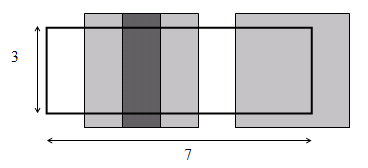
\includegraphics[width=0.7\textwidth]{../latex/img/1014/1014-1.png}
\caption{บริเวณกรอบสีดำหนาคือหน้าต่าง และส่วนที่เป็นสีเทาคือบริเวณที่ม่านสามารถบังแดดไว้ได้}
\end{figure}
\bigskip
\underline{\textbf{โจทย์}}  จงเขียนโปรแกรมเพื่อรับข้อมูลขนาดของหน้าต่างและการแขวนผ้าม่าน จากนั้นคำนวณหาพื้นที่ของหน้าต่างที่ไม่โดนม่านบัง (แสงผ่านได้ $100\%$) และพื้นที่ที่แสงสามารถส่องผ่านได้ $50\%$ มีหน่วยเป็นตารางเมตร

\InputFile

\textbf{บรรทัดแรก} รับจำนวนเต็มสามจำนวน $W$ $H$ $n$ $(1\leq W\leq 3\,000; 1 \leq H\leq 10; 1\leq n\leq 100)$

\newpage

\textbf{บรรทัดที่ $2$ ถึง $n+1$ }บรรทัดที่ $i+1$ จะรับข้อมูลม่านผืนที่ $i$ โดยแต่ละบรรทัดจะประกอบด้วย จำนวนเต็มสองจำนวน $x$ $a$ $(0\leq x \leq W ; 1\leq a \leq 1\,000)$ โดย $x$ แทนตำแหน่งนับจากขอบหน้าต่างด้านซ้ายที่เริ่มแขวนผ้าม่าน และ $a$ แทนความกว้างของผ้าม่าน ทั้ง $a$ และ $x$ มีหน่วยเป็นเมตร ผ้าม่านจะบังแดดจากหน้าต่างเริ่มจากขอบด้านซ้าย $x$ เมตรถึง $x + a$ เมตร

\OutputFile

\textbf{มีบรรทัดเดียว} ประกอบด้วยจำนวนเต็มสองค่า ตัวแรกเป็นพื้นที่ของหน้าต่างที่แสงส่องผ่านได้โดยไม่โดนม่านบัง (แสงผ่านได้ $100\%$) ตัวที่สองเป็นพื้นที่ของหน้าต่างที่แสงส่องผ่านได้ $50\%$

\Examples

\begin{example}
\exmp{7 3 3
1 2
5 3
2 2}{6 12}%
\end{example}


\Source

การแข่งขันคอมพิวเตอร์โอลิมปิก สอวน. ครั้งที่ 3 มหาวิทยาลัยขอนแก่น

\end{problem}

\end{document}